\documentclass[1p]{elsarticle_modified}
%\bibliographystyle{elsarticle-num}

%\usepackage[colorlinks]{hyperref}
%\usepackage{abbrmath_seonhwa} %\Abb, \Ascr, \Acal ,\Abf, \Afrak
\usepackage{amsfonts}
\usepackage{amssymb}
\usepackage{amsmath}
\usepackage{amsthm}
\usepackage{scalefnt}
\usepackage{amsbsy}
\usepackage{kotex}
\usepackage{caption}
\usepackage{subfig}
\usepackage{color}
\usepackage{graphicx}
\usepackage{xcolor} %% white, black, red, green, blue, cyan, magenta, yellow
\usepackage{float}
\usepackage{setspace}
\usepackage{hyperref}

\usepackage{tikz}
\usetikzlibrary{arrows}

\usepackage{multirow}
\usepackage{array} % fixed length table
\usepackage{hhline}

%%%%%%%%%%%%%%%%%%%%%
\makeatletter
\renewcommand*\env@matrix[1][\arraystretch]{%
	\edef\arraystretch{#1}%
	\hskip -\arraycolsep
	\let\@ifnextchar\new@ifnextchar
	\array{*\c@MaxMatrixCols c}}
\makeatother %https://tex.stackexchange.com/questions/14071/how-can-i-increase-the-line-spacing-in-a-matrix
%%%%%%%%%%%%%%%

\usepackage[normalem]{ulem}

\newcommand{\msout}[1]{\ifmmode\text{\sout{\ensuremath{#1}}}\else\sout{#1}\fi}
%SOURCE: \msout is \stkout macro in https://tex.stackexchange.com/questions/20609/strikeout-in-math-mode

\newcommand{\cancel}[1]{
	\ifmmode
	{\color{red}\msout{#1}}
	\else
	{\color{red}\sout{#1}}
	\fi
}

\newcommand{\add}[1]{
	{\color{blue}\uwave{#1}}
}

\newcommand{\replace}[2]{
	\ifmmode
	{\color{red}\msout{#1}}{\color{blue}\uwave{#2}}
	\else
	{\color{red}\sout{#1}}{\color{blue}\uwave{#2}}
	\fi
}

\newcommand{\Sol}{\mathcal{S}} %segment
\newcommand{\D}{D} %diagram
\newcommand{\A}{\mathcal{A}} %arc


%%%%%%%%%%%%%%%%%%%%%%%%%%%%%5 test

\def\sl{\operatorname{\textup{SL}}(2,\Cbb)}
\def\psl{\operatorname{\textup{PSL}}(2,\Cbb)}
\def\quan{\mkern 1mu \triangleright \mkern 1mu}

\theoremstyle{definition}
\newtheorem{thm}{Theorem}[section]
\newtheorem{prop}[thm]{Proposition}
\newtheorem{lem}[thm]{Lemma}
\newtheorem{ques}[thm]{Question}
\newtheorem{cor}[thm]{Corollary}
\newtheorem{defn}[thm]{Definition}
\newtheorem{exam}[thm]{Example}
\newtheorem{rmk}[thm]{Remark}
\newtheorem{alg}[thm]{Algorithm}

\newcommand{\I}{\sqrt{-1}}
\begin{document}

%\begin{frontmatter}
%
%\title{Boundary parabolic representations of knots up to 8 crossings}
%
%%% Group authors per affiliation:
%\author{Yunhi Cho} 
%\address{Department of Mathematics, University of Seoul, Seoul, Korea}
%\ead{yhcho@uos.ac.kr}
%
%
%\author{Seonhwa Kim} %\fnref{s_kim}}
%\address{Center for Geometry and Physics, Institute for Basic Science, Pohang, 37673, Korea}
%\ead{ryeona17@ibs.re.kr}
%
%\author{Hyuk Kim}
%\address{Department of Mathematical Sciences, Seoul National University, Seoul 08826, Korea}
%\ead{hyukkim@snu.ac.kr}
%
%\author{Seokbeom Yoon}
%\address{Department of Mathematical Sciences, Seoul National University, Seoul, 08826,  Korea}
%\ead{sbyoon15@snu.ac.kr}
%
%\begin{abstract}
%We find all boundary parabolic representation of knots up to 8 crossings.
%
%\end{abstract}
%\begin{keyword}
%    \MSC[2010] 57M25 
%\end{keyword}
%
%\end{frontmatter}

%\linenumbers
%\tableofcontents
%
\newcommand\colored[1]{\textcolor{white}{\rule[-0.35ex]{0.8em}{1.4ex}}\kern-0.8em\color{red} #1}%
%\newcommand\colored[1]{\textcolor{white}{ #1}\kern-2.17ex	\textcolor{white}{ #1}\kern-1.81ex	\textcolor{white}{ #1}\kern-2.15ex\color{red}#1	}

{\Large $\underline{11n_{175}~(K11n_{175})}$}

\setlength{\tabcolsep}{10pt}
\renewcommand{\arraystretch}{1.6}
\vspace{1cm}\begin{tabular}{m{100pt}>{\centering\arraybackslash}m{274pt}}
\multirow{5}{120pt}{
	\centering
	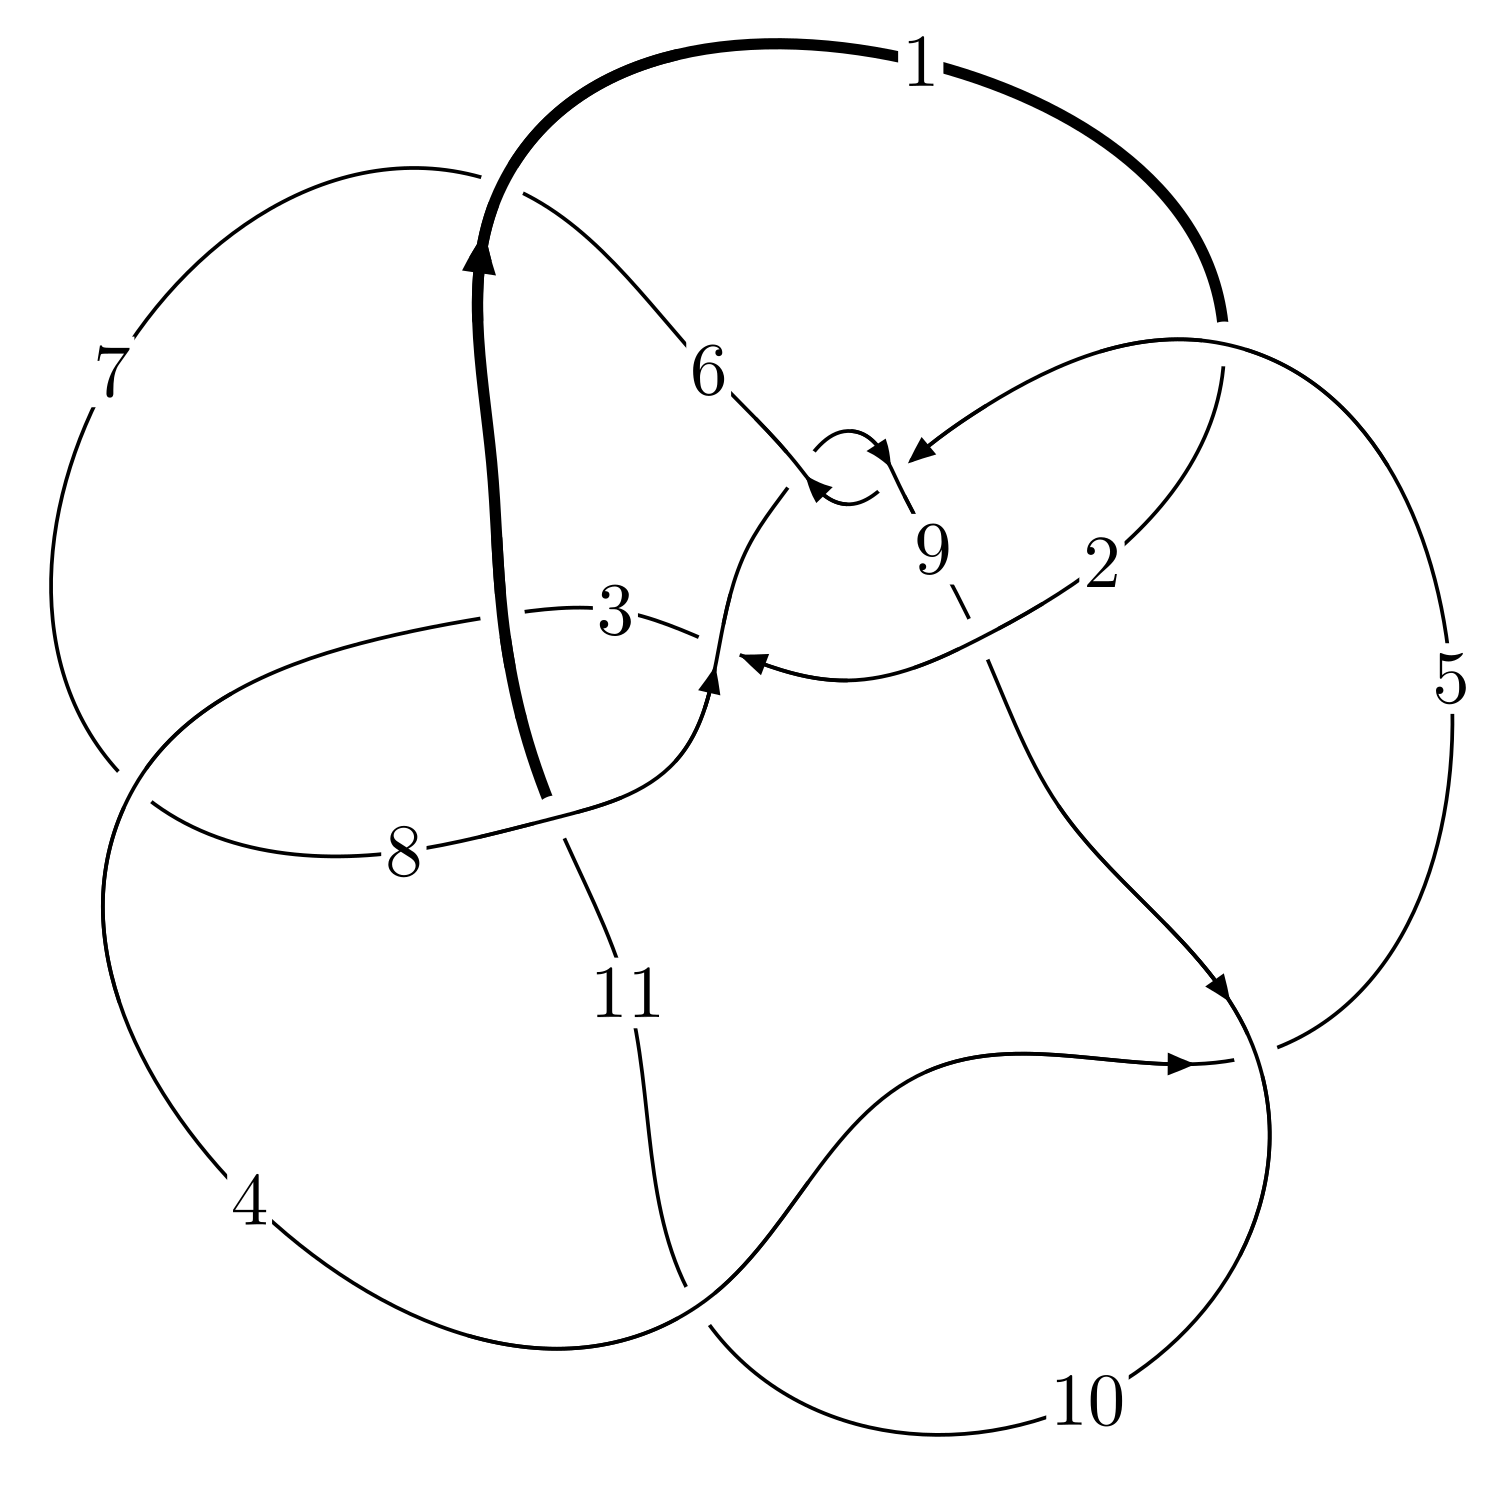
\includegraphics[width=112pt]{../../../GIT/diagram.site/Diagrams/png/791_11n_175.png}\\
\ \ \ A knot diagram\footnotemark}&
\allowdisplaybreaks
\textbf{Linearized knot diagam} \\
\cline{2-2}
 &
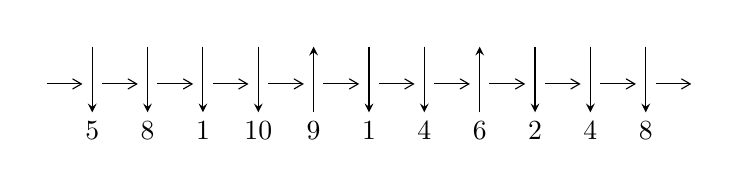
\begin{tikzpicture}[x=20pt, y=17pt]
	% nodes
	\node (C0) at (0, 0) {};
	\node (C1) at (1, 0) {};
	\node (C1U) at (1, +1) {};
	\node (C1D) at (1, -1) {5};

	\node (C2) at (2, 0) {};
	\node (C2U) at (2, +1) {};
	\node (C2D) at (2, -1) {8};

	\node (C3) at (3, 0) {};
	\node (C3U) at (3, +1) {};
	\node (C3D) at (3, -1) {1};

	\node (C4) at (4, 0) {};
	\node (C4U) at (4, +1) {};
	\node (C4D) at (4, -1) {10};

	\node (C5) at (5, 0) {};
	\node (C5U) at (5, +1) {};
	\node (C5D) at (5, -1) {9};

	\node (C6) at (6, 0) {};
	\node (C6U) at (6, +1) {};
	\node (C6D) at (6, -1) {1};

	\node (C7) at (7, 0) {};
	\node (C7U) at (7, +1) {};
	\node (C7D) at (7, -1) {4};

	\node (C8) at (8, 0) {};
	\node (C8U) at (8, +1) {};
	\node (C8D) at (8, -1) {6};

	\node (C9) at (9, 0) {};
	\node (C9U) at (9, +1) {};
	\node (C9D) at (9, -1) {2};

	\node (C10) at (10, 0) {};
	\node (C10U) at (10, +1) {};
	\node (C10D) at (10, -1) {4};

	\node (C11) at (11, 0) {};
	\node (C11U) at (11, +1) {};
	\node (C11D) at (11, -1) {8};
	\node (C12) at (12, 0) {};

	% arrows
	\draw[->,>={angle 60}]
	(C0) edge (C1) (C1) edge (C2) (C2) edge (C3) (C3) edge (C4) (C4) edge (C5) (C5) edge (C6) (C6) edge (C7) (C7) edge (C8) (C8) edge (C9) (C9) edge (C10) (C10) edge (C11) (C11) edge (C12) ;	\draw[->,>=stealth]
	(C1U) edge (C1D) (C2U) edge (C2D) (C3U) edge (C3D) (C4U) edge (C4D) (C5D) edge (C5U) (C6U) edge (C6D) (C7U) edge (C7D) (C8D) edge (C8U) (C9U) edge (C9D) (C10U) edge (C10D) (C11U) edge (C11D) ;
	\end{tikzpicture} \\
\hhline{~~} \\& 
\textbf{Solving Sequence} \\ \cline{2-2} 
 &
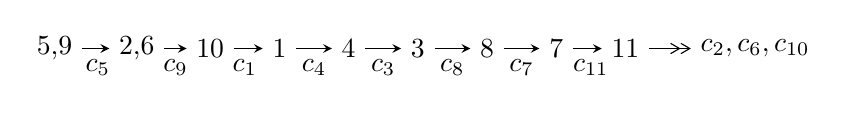
\begin{tikzpicture}[x=25pt, y=7pt]
	% node
	\node (A0) at (-1/8, 0) {5,9};
	\node (A1) at (17/16, 0) {2,6};
	\node (A2) at (17/8, 0) {10};
	\node (A3) at (25/8, 0) {1};
	\node (A4) at (33/8, 0) {4};
	\node (A5) at (41/8, 0) {3};
	\node (A6) at (49/8, 0) {8};
	\node (A7) at (57/8, 0) {7};
	\node (A8) at (65/8, 0) {11};
	\node (C1) at (1/2, -1) {$c_{5}$};
	\node (C2) at (13/8, -1) {$c_{9}$};
	\node (C3) at (21/8, -1) {$c_{1}$};
	\node (C4) at (29/8, -1) {$c_{4}$};
	\node (C5) at (37/8, -1) {$c_{3}$};
	\node (C6) at (45/8, -1) {$c_{8}$};
	\node (C7) at (53/8, -1) {$c_{7}$};
	\node (C8) at (61/8, -1) {$c_{11}$};
	\node (A9) at (10, 0) {$c_{2},c_{6},c_{10}$};

	% edge
	\draw[->,>=stealth]	
	(A0) edge (A1) (A1) edge (A2) (A2) edge (A3) (A3) edge (A4) (A4) edge (A5) (A5) edge (A6) (A6) edge (A7) (A7) edge (A8) ;
	\draw[->>,>={angle 60}]	
	(A8) edge (A9);
\end{tikzpicture} \\ 

\end{tabular} \\

\footnotetext{
The image of knot diagram is generated by the software ``\textbf{Draw programme}" developed by Andrew Bartholomew(\url{http://www.layer8.co.uk/maths/draw/index.htm\#Running-draw}), where we modified some parts for our purpose(\url{https://github.com/CATsTAILs/LinksPainter}).
}\phantom \\ \newline 
\centering \textbf{Ideals for irreducible components\footnotemark of $X_{\text{par}}$} 
 
\begin{align*}
I^u_{1}&=\langle 
3 u^{17}-27 u^{16}+\cdots+2 b-4,\;- u^{17}+6 u^{16}+\cdots+2 a-35,\;u^{18}-9 u^{17}+\cdots-50 u+4\rangle \\
I^u_{2}&=\langle 
-43 u^5 a^3+57 u^5 a^2+\cdots+93 a+11,\;- u^5 a^3-3 u^5 a+\cdots-8 a+28,\;u^6+u^5+3 u^4+2 u^3+2 u^2+u-1\rangle \\
I^u_{3}&=\langle 
- u^8- u^7-3 u^6-2 u^5-4 u^4-3 u^3-3 u^2+b-2 u-1,\\
\phantom{I^u_{3}}&\phantom{= \langle  }u^9+2 u^8+3 u^7+5 u^6+4 u^5+8 u^4+3 u^3+5 u^2+3 a+u+1,\\
\phantom{I^u_{3}}&\phantom{= \langle  }u^{10}+2 u^9+6 u^8+8 u^7+13 u^6+14 u^5+15 u^4+14 u^3+10 u^2+7 u+3\rangle \\
\\
\end{align*}
\raggedright * 3 irreducible components of $\dim_{\mathbb{C}}=0$, with total 52 representations.\\
\footnotetext{All coefficients of polynomials are rational numbers. But the coefficients are sometimes approximated in decimal forms when there is not enough margin.}
\newpage
\renewcommand{\arraystretch}{1}
\centering \section*{I. $I^u_{1}= \langle 3 u^{17}-27 u^{16}+\cdots+2 b-4,\;- u^{17}+6 u^{16}+\cdots+2 a-35,\;u^{18}-9 u^{17}+\cdots-50 u+4 \rangle$}
\flushleft \textbf{(i) Arc colorings}\\
\begin{tabular}{m{7pt} m{180pt} m{7pt} m{180pt} }
\flushright $a_{5}=$&$\begin{pmatrix}1\\0\end{pmatrix}$ \\
\flushright $a_{9}=$&$\begin{pmatrix}0\\u\end{pmatrix}$ \\
\flushright $a_{2}=$&$\begin{pmatrix}\frac{1}{2} u^{17}-3 u^{16}+\cdots-\frac{273}{2} u+\frac{35}{2}\\-\frac{3}{2} u^{17}+\frac{27}{2} u^{16}+\cdots-\frac{85}{2} u+2\end{pmatrix}$ \\
\flushright $a_{6}=$&$\begin{pmatrix}1\\- u^2\end{pmatrix}$ \\
\flushright $a_{10}=$&$\begin{pmatrix}\frac{9}{4} u^{17}-\frac{75}{4} u^{16}+\cdots+\frac{731}{4} u-18\\-\frac{3}{2} u^{17}+\frac{25}{2} u^{16}+\cdots-\frac{187}{2} u+9\end{pmatrix}$ \\
\flushright $a_{1}=$&$\begin{pmatrix}- u^{17}+\frac{21}{2} u^{16}+\cdots-179 u+\frac{39}{2}\\-\frac{3}{2} u^{17}+\frac{27}{2} u^{16}+\cdots-\frac{85}{2} u+2\end{pmatrix}$ \\
\flushright $a_{4}=$&$\begin{pmatrix}- u^{17}+\frac{19}{2} u^{16}+\cdots-261 u+\frac{55}{2}\\\frac{1}{2} u^{17}-\frac{7}{2} u^{16}+\cdots+\frac{179}{2} u-10\end{pmatrix}$ \\
\flushright $a_{3}=$&$\begin{pmatrix}-\frac{3}{2} u^{17}+14 u^{16}+\cdots-\frac{331}{2} u+\frac{39}{2}\\-\frac{3}{2} u^{17}+\frac{25}{2} u^{16}+\cdots+\frac{57}{2} u-4\end{pmatrix}$ \\
\flushright $a_{8}=$&$\begin{pmatrix}- u\\u^3+u\end{pmatrix}$ \\
\flushright $a_{7}=$&$\begin{pmatrix}\frac{5}{4} u^{17}-\frac{43}{4} u^{16}+\cdots+\frac{327}{4} u-7\\-\frac{1}{2} u^{17}+\frac{9}{2} u^{16}+\cdots-\frac{145}{2} u+7\end{pmatrix}$ \\
\flushright $a_{11}=$&$\begin{pmatrix}- u^{17}+\frac{21}{2} u^{16}+\cdots-198 u+\frac{43}{2}\\-\frac{3}{2} u^{17}+\frac{27}{2} u^{16}+\cdots+194 u^2-\frac{47}{2} u\end{pmatrix}$\\ \flushright $a_{11}=$&$\begin{pmatrix}- u^{17}+\frac{21}{2} u^{16}+\cdots-198 u+\frac{43}{2}\\-\frac{3}{2} u^{17}+\frac{27}{2} u^{16}+\cdots+194 u^2-\frac{47}{2} u\end{pmatrix}$\\&\end{tabular}
\flushleft \textbf{(ii) Obstruction class $= -1$}\\~\\
\flushleft \textbf{(iii) Cusp Shapes $= -3 u^{17}+27 u^{16}-140 u^{15}+513 u^{14}-1455 u^{13}+3348 u^{12}-6412 u^{11}+10399 u^{10}-14401 u^9+17095 u^8-17369 u^7+14980 u^6-10819 u^5+6362 u^4-2908 u^3+949 u^2-170 u-2$}\\~\\
\newpage\renewcommand{\arraystretch}{1}
\flushleft \textbf{(iv) u-Polynomials at the component}\newline \\
\begin{tabular}{m{50pt}|m{274pt}}
Crossings & \hspace{64pt}u-Polynomials at each crossing \\
\hline $$\begin{aligned}c_{1},c_{9}\end{aligned}$$&$\begin{aligned}
&u^{18}-2 u^{16}+\cdots+7 u^2-1
\end{aligned}$\\
\hline $$\begin{aligned}c_{2},c_{6}\end{aligned}$$&$\begin{aligned}
&u^{18}-7 u^{16}+\cdots-2 u-13
\end{aligned}$\\
\hline $$\begin{aligned}c_{3}\end{aligned}$$&$\begin{aligned}
&u^{18}-13 u^{17}+\cdots-62 u-52
\end{aligned}$\\
\hline $$\begin{aligned}c_{4},c_{10}\end{aligned}$$&$\begin{aligned}
&u^{18}+13 u^{17}+\cdots+608 u+64
\end{aligned}$\\
\hline $$\begin{aligned}c_{5},c_{8}\end{aligned}$$&$\begin{aligned}
&u^{18}+9 u^{17}+\cdots+50 u+4
\end{aligned}$\\
\hline $$\begin{aligned}c_{7},c_{11}\end{aligned}$$&$\begin{aligned}
&u^{18}+2 u^{17}+\cdots+u+1
\end{aligned}$\\
\hline
\end{tabular}\\~\\
\newpage\renewcommand{\arraystretch}{1}
\flushleft \textbf{(v) Riley Polynomials at the component}\newline \\
\begin{tabular}{m{50pt}|m{274pt}}
Crossings & \hspace{64pt}Riley Polynomials at each crossing \\
\hline $$\begin{aligned}c_{1},c_{9}\end{aligned}$$&$\begin{aligned}
&y^{18}-4 y^{17}+\cdots-14 y+1
\end{aligned}$\\
\hline $$\begin{aligned}c_{2},c_{6}\end{aligned}$$&$\begin{aligned}
&y^{18}-14 y^{17}+\cdots-1564 y+169
\end{aligned}$\\
\hline $$\begin{aligned}c_{3}\end{aligned}$$&$\begin{aligned}
&y^{18}-19 y^{17}+\cdots+6660 y+2704
\end{aligned}$\\
\hline $$\begin{aligned}c_{4},c_{10}\end{aligned}$$&$\begin{aligned}
&y^{18}+9 y^{17}+\cdots-17408 y+4096
\end{aligned}$\\
\hline $$\begin{aligned}c_{5},c_{8}\end{aligned}$$&$\begin{aligned}
&y^{18}+13 y^{17}+\cdots-364 y+16
\end{aligned}$\\
\hline $$\begin{aligned}c_{7},c_{11}\end{aligned}$$&$\begin{aligned}
&y^{18}-26 y^{17}+\cdots-21 y+1
\end{aligned}$\\
\hline
\end{tabular}\\~\\
\newpage\flushleft \textbf{(vi) Complex Volumes and Cusp Shapes}
$$\begin{array}{c|c|c}  
\text{Solutions to }I^u_{1}& \I (\text{vol} + \sqrt{-1}CS) & \text{Cusp shape}\\
 \hline 
\begin{aligned}
u &= \phantom{-}1.082250 + 0.227691 I \\
a &= \phantom{-}0.552560 - 1.011470 I \\
b &= -0.828307 + 0.968844 I\end{aligned}
 & -2.96562 + 8.53890 I & -6.56006 - 6.26417 I \\ \hline\begin{aligned}
u &= \phantom{-}1.082250 - 0.227691 I \\
a &= \phantom{-}0.552560 + 1.011470 I \\
b &= -0.828307 - 0.968844 I\end{aligned}
 & -2.96562 - 8.53890 I & -6.56006 + 6.26417 I \\ \hline\begin{aligned}
u &= -0.118459 + 1.148360 I \\
a &= \phantom{-}0.235904 + 0.462260 I \\
b &= \phantom{-}0.558784 - 0.216142 I\end{aligned}
 & -1.23970 - 1.97493 I & -7.15329 + 4.18348 I \\ \hline\begin{aligned}
u &= -0.118459 - 1.148360 I \\
a &= \phantom{-}0.235904 - 0.462260 I \\
b &= \phantom{-}0.558784 + 0.216142 I\end{aligned}
 & -1.23970 + 1.97493 I & -7.15329 - 4.18348 I \\ \hline\begin{aligned}
u &= \phantom{-}0.119333 + 1.157960 I \\
a &= -0.466244 - 0.909025 I \\
b &= -0.996978 + 0.648369 I\end{aligned}
 & -3.72560 + 1.35027 I & -12.38494 - 1.13112 I \\ \hline\begin{aligned}
u &= \phantom{-}0.119333 - 1.157960 I \\
a &= -0.466244 + 0.909025 I \\
b &= -0.996978 - 0.648369 I\end{aligned}
 & -3.72560 - 1.35027 I & -12.38494 + 1.13112 I \\ \hline\begin{aligned}
u &= \phantom{-}0.200699 + 1.177200 I \\
a &= \phantom{-}0.746983 + 1.092830 I \\
b &= \phantom{-}1.13656 - 1.09868 I\end{aligned}
 & \phantom{-}0.82240 + 4.90619 I & -8.42983 - 0.71625 I \\ \hline\begin{aligned}
u &= \phantom{-}0.200699 - 1.177200 I \\
a &= \phantom{-}0.746983 - 1.092830 I \\
b &= \phantom{-}1.13656 + 1.09868 I\end{aligned}
 & \phantom{-}0.82240 - 4.90619 I & -8.42983 + 0.71625 I \\ \hline\begin{aligned}
u &= \phantom{-}1.48738\phantom{ +0.000000I} \\
a &= -0.407205\phantom{ +0.000000I} \\
b &= \phantom{-}0.605669\phantom{ +0.000000I}\end{aligned}
 & -6.56717\phantom{ +0.000000I} & -21.0980\phantom{ +0.000000I} \\ \hline\begin{aligned}
u &= \phantom{-}0.46203 + 1.43201 I \\
a &= -0.460365 - 1.018170 I \\
b &= -1.24533 + 1.12967 I\end{aligned}
 & -8.1698 + 13.9821 I & -9.44231 - 6.99967 I\\
 \hline 
 \end{array}$$\newpage$$\begin{array}{c|c|c}  
\text{Solutions to }I^u_{1}& \I (\text{vol} + \sqrt{-1}CS) & \text{Cusp shape}\\
 \hline 
\begin{aligned}
u &= \phantom{-}0.46203 - 1.43201 I \\
a &= -0.460365 + 1.018170 I \\
b &= -1.24533 - 1.12967 I\end{aligned}
 & -8.1698 - 13.9821 I & -9.44231 + 6.99967 I \\ \hline\begin{aligned}
u &= \phantom{-}0.446331 + 0.206443 I \\
a &= -1.97819 - 0.97124 I \\
b &= \phantom{-}0.682422 + 0.841875 I\end{aligned}
 & \phantom{-}3.74044 - 2.38337 I & -9.76739 + 4.47048 I \\ \hline\begin{aligned}
u &= \phantom{-}0.446331 - 0.206443 I \\
a &= -1.97819 + 0.97124 I \\
b &= \phantom{-}0.682422 - 0.841875 I\end{aligned}
 & \phantom{-}3.74044 + 2.38337 I & -9.76739 - 4.47048 I \\ \hline\begin{aligned}
u &= \phantom{-}0.51935 + 1.48126 I \\
a &= \phantom{-}0.115710 + 0.783531 I \\
b &= \phantom{-}1.100520 - 0.578325 I\end{aligned}
 & -11.82300 + 6.66028 I & -12.41949 - 4.41908 I \\ \hline\begin{aligned}
u &= \phantom{-}0.51935 - 1.48126 I \\
a &= \phantom{-}0.115710 - 0.783531 I \\
b &= \phantom{-}1.100520 + 0.578325 I\end{aligned}
 & -11.82300 - 6.66028 I & -12.41949 + 4.41908 I \\ \hline\begin{aligned}
u &= \phantom{-}0.93646 + 1.42974 I \\
a &= \phantom{-}0.302389 - 0.123907 I \\
b &= -0.460331 - 0.316302 I\end{aligned}
 & -5.89009 - 1.65718 I & -15.9057 + 11.0160 I \\ \hline\begin{aligned}
u &= \phantom{-}0.93646 - 1.42974 I \\
a &= \phantom{-}0.302389 + 0.123907 I \\
b &= -0.460331 + 0.316302 I\end{aligned}
 & -5.89009 + 1.65718 I & -15.9057 - 11.0160 I \\ \hline\begin{aligned}
u &= \phantom{-}0.216637\phantom{ +0.000000I} \\
a &= \phantom{-}2.30970\phantom{ +0.000000I} \\
b &= -0.500367\phantom{ +0.000000I}\end{aligned}
 & -0.728249\phantom{ +0.000000I} & -13.7760\phantom{ +0.000000I}\\
 \hline 
 \end{array}$$\newpage\newpage\renewcommand{\arraystretch}{1}
\centering \section*{II. $I^u_{2}= \langle -43 u^5 a^3+57 u^5 a^2+\cdots+93 a+11,\;- u^5 a^3-3 u^5 a+\cdots-8 a+28,\;u^6+u^5+3 u^4+2 u^3+2 u^2+u-1 \rangle$}
\flushleft \textbf{(i) Arc colorings}\\
\begin{tabular}{m{7pt} m{180pt} m{7pt} m{180pt} }
\flushright $a_{5}=$&$\begin{pmatrix}1\\0\end{pmatrix}$ \\
\flushright $a_{9}=$&$\begin{pmatrix}0\\u\end{pmatrix}$ \\
\flushright $a_{2}=$&$\begin{pmatrix}a\\0.394495 a^{3} u^{5}-0.522936 a^{2} u^{5}+\cdots-0.853211 a-0.100917\end{pmatrix}$ \\
\flushright $a_{6}=$&$\begin{pmatrix}1\\- u^2\end{pmatrix}$ \\
\flushright $a_{10}=$&$\begin{pmatrix}- a^2 u\\0.385321 a^{3} u^{5}-0.394495 a^{2} u^{5}+\cdots+0.724771 a-0.935780\end{pmatrix}$ \\
\flushright $a_{1}=$&$\begin{pmatrix}0.394495 a^{3} u^{5}-0.522936 a^{2} u^{5}+\cdots+0.146789 a-0.100917\\0.394495 a^{3} u^{5}-0.522936 a^{2} u^{5}+\cdots-0.853211 a-0.100917\end{pmatrix}$ \\
\flushright $a_{4}=$&$\begin{pmatrix}0.321101 a^{3} u^{5}-0.495413 a^{2} u^{5}+\cdots-0.229358 a+0.220183\\0.385321 a^{3} u^{5}-0.394495 a^{2} u^{5}+\cdots+0.724771 a+0.0642202\end{pmatrix}$ \\
\flushright $a_{3}=$&$\begin{pmatrix}0.798165 a^{3} u^{5}-1.17431 a^{2} u^{5}+\cdots+0.715596 a-0.366972\\0.862385 a^{3} u^{5}-1.07339 a^{2} u^{5}+\cdots+0.669725 a-0.522936\end{pmatrix}$ \\
\flushright $a_{8}=$&$\begin{pmatrix}- u\\u^3+u\end{pmatrix}$ \\
\flushright $a_{7}=$&$\begin{pmatrix}0.522936 a^{3} u^{5}-1.32110 a^{2} u^{5}+\cdots+0.0550459 a+2.58716\\0.146789 a^{3} u^{5}-1.05505 a^{2} u^{5}+\cdots+0.752294 a-0.642202\end{pmatrix}$ \\
\flushright $a_{11}=$&$\begin{pmatrix}0.0642202 a^{3} u^{5}+0.100917 a^{2} u^{5}+\cdots+0.954128 a-0.155963\\-0.385321 a^{3} u^{5}+0.394495 a^{2} u^{5}+\cdots-0.724771 a-0.0642202\end{pmatrix}$\\ \flushright $a_{11}=$&$\begin{pmatrix}0.0642202 a^{3} u^{5}+0.100917 a^{2} u^{5}+\cdots+0.954128 a-0.155963\\-0.385321 a^{3} u^{5}+0.394495 a^{2} u^{5}+\cdots-0.724771 a-0.0642202\end{pmatrix}$\\&\end{tabular}
\flushleft \textbf{(ii) Obstruction class $= -1$}\\~\\
\flushleft \textbf{(iii) Cusp Shapes $= -\frac{168}{109} u^5 a^3+\frac{172}{109} u^5 a^2+\cdots-\frac{316}{109} a-\frac{682}{109}$}\\~\\
\newpage\renewcommand{\arraystretch}{1}
\flushleft \textbf{(iv) u-Polynomials at the component}\newline \\
\begin{tabular}{m{50pt}|m{274pt}}
Crossings & \hspace{64pt}u-Polynomials at each crossing \\
\hline $$\begin{aligned}c_{1},c_{9}\end{aligned}$$&$\begin{aligned}
&u^{24}+5 u^{23}+\cdots-12 u+3
\end{aligned}$\\
\hline $$\begin{aligned}c_{2},c_{6}\end{aligned}$$&$\begin{aligned}
&u^{24}- u^{23}+\cdots-1976 u+793
\end{aligned}$\\
\hline $$\begin{aligned}c_{3}\end{aligned}$$&$\begin{aligned}
&(u^6+5 u^5+7 u^4-2 u^2+3 u-1)^4
\end{aligned}$\\
\hline $$\begin{aligned}c_{4},c_{10}\end{aligned}$$&$\begin{aligned}
&(u^2- u+1)^{12}
\end{aligned}$\\
\hline $$\begin{aligned}c_{5},c_{8}\end{aligned}$$&$\begin{aligned}
&(u^6- u^5+3 u^4-2 u^3+2 u^2- u-1)^4
\end{aligned}$\\
\hline $$\begin{aligned}c_{7},c_{11}\end{aligned}$$&$\begin{aligned}
&u^{24}+u^{23}+\cdots+198 u+93
\end{aligned}$\\
\hline
\end{tabular}\\~\\
\newpage\renewcommand{\arraystretch}{1}
\flushleft \textbf{(v) Riley Polynomials at the component}\newline \\
\begin{tabular}{m{50pt}|m{274pt}}
Crossings & \hspace{64pt}Riley Polynomials at each crossing \\
\hline $$\begin{aligned}c_{1},c_{9}\end{aligned}$$&$\begin{aligned}
&y^{24}+3 y^{23}+\cdots-156 y+9
\end{aligned}$\\
\hline $$\begin{aligned}c_{2},c_{6}\end{aligned}$$&$\begin{aligned}
&y^{24}-17 y^{23}+\cdots-2553304 y+628849
\end{aligned}$\\
\hline $$\begin{aligned}c_{3}\end{aligned}$$&$\begin{aligned}
&(y^6-11 y^5+45 y^4-60 y^3-10 y^2-5 y+1)^4
\end{aligned}$\\
\hline $$\begin{aligned}c_{4},c_{10}\end{aligned}$$&$\begin{aligned}
&(y^2+y+1)^{12}
\end{aligned}$\\
\hline $$\begin{aligned}c_{5},c_{8}\end{aligned}$$&$\begin{aligned}
&(y^6+5 y^5+9 y^4+4 y^3-6 y^2-5 y+1)^4
\end{aligned}$\\
\hline $$\begin{aligned}c_{7},c_{11}\end{aligned}$$&$\begin{aligned}
&y^{24}-25 y^{23}+\cdots+40776 y+8649
\end{aligned}$\\
\hline
\end{tabular}\\~\\
\newpage\flushleft \textbf{(vi) Complex Volumes and Cusp Shapes}
$$\begin{array}{c|c|c}  
\text{Solutions to }I^u_{2}& \I (\text{vol} + \sqrt{-1}CS) & \text{Cusp shape}\\
 \hline 
\begin{aligned}
u &= -0.873214\phantom{ +0.000000I} \\
a &= \phantom{-}0.696693 + 0.745196 I \\
b &= -0.424035 - 0.969980 I\end{aligned}
 & \phantom{-}2.72528 - 2.02988 I & -5.73050 + 3.46410 I \\ \hline\begin{aligned}
u &= -0.873214\phantom{ +0.000000I} \\
a &= \phantom{-}0.696693 - 0.745196 I \\
b &= -0.424035 + 0.969980 I\end{aligned}
 & \phantom{-}2.72528 + 2.02988 I & -5.73050 - 3.46410 I \\ \hline\begin{aligned}
u &= -0.873214\phantom{ +0.000000I} \\
a &= -0.485602 + 1.110820 I \\
b &= \phantom{-}0.608362 - 0.650716 I\end{aligned}
 & \phantom{-}2.72528 + 2.02988 I & -5.73050 - 3.46410 I \\ \hline\begin{aligned}
u &= -0.873214\phantom{ +0.000000I} \\
a &= -0.485602 - 1.110820 I \\
b &= \phantom{-}0.608362 + 0.650716 I\end{aligned}
 & \phantom{-}2.72528 - 2.02988 I & -5.73050 + 3.46410 I \\ \hline\begin{aligned}
u &= \phantom{-}0.138835 + 1.234450 I \\
a &= \phantom{-}0.047053 - 0.843430 I \\
b &= \phantom{-}0.49525 + 2.03273 I\end{aligned}
 & -7.89505 - 0.05747 I & -13.42428 - 0.22068 I \\ \hline\begin{aligned}
u &= \phantom{-}0.138835 + 1.234450 I \\
a &= -1.67067 + 0.21330 I \\
b &= -1.047700 + 0.059012 I\end{aligned}
 & -7.89505 - 0.05747 I & -13.42428 - 0.22068 I \\ \hline\begin{aligned}
u &= \phantom{-}0.138835 + 1.234450 I \\
a &= \phantom{-}0.010113 + 0.251086 I \\
b &= -1.84383 - 1.47696 I\end{aligned}
 & -7.89505 + 4.00229 I & -13.4243 - 7.1489 I \\ \hline\begin{aligned}
u &= \phantom{-}0.138835 + 1.234450 I \\
a &= \phantom{-}1.34740 - 1.34211 I \\
b &= \phantom{-}0.308548 - 0.047344 I\end{aligned}
 & -7.89505 + 4.00229 I & -13.4243 - 7.1489 I \\ \hline\begin{aligned}
u &= \phantom{-}0.138835 - 1.234450 I \\
a &= \phantom{-}0.047053 + 0.843430 I \\
b &= \phantom{-}0.49525 - 2.03273 I\end{aligned}
 & -7.89505 + 0.05747 I & -13.42428 + 0.22068 I \\ \hline\begin{aligned}
u &= \phantom{-}0.138835 - 1.234450 I \\
a &= -1.67067 - 0.21330 I \\
b &= -1.047700 - 0.059012 I\end{aligned}
 & -7.89505 + 0.05747 I & -13.42428 + 0.22068 I\\
 \hline 
 \end{array}$$\newpage$$\begin{array}{c|c|c}  
\text{Solutions to }I^u_{2}& \I (\text{vol} + \sqrt{-1}CS) & \text{Cusp shape}\\
 \hline 
\begin{aligned}
u &= \phantom{-}0.138835 - 1.234450 I \\
a &= \phantom{-}0.010113 - 0.251086 I \\
b &= -1.84383 + 1.47696 I\end{aligned}
 & -7.89505 - 4.00229 I & -13.4243 + 7.1489 I \\ \hline\begin{aligned}
u &= \phantom{-}0.138835 - 1.234450 I \\
a &= \phantom{-}1.34740 + 1.34211 I \\
b &= \phantom{-}0.308548 + 0.047344 I\end{aligned}
 & -7.89505 - 4.00229 I & -13.4243 + 7.1489 I \\ \hline\begin{aligned}
u &= -0.408802 + 1.276380 I \\
a &= -0.353289 + 0.834565 I \\
b &= -1.20721 - 1.28821 I\end{aligned}
 & -1.23922 - 6.62201 I & -9.41886 + 6.66892 I \\ \hline\begin{aligned}
u &= -0.408802 + 1.276380 I \\
a &= -0.070379 + 0.682688 I \\
b &= -0.269751 - 0.368903 I\end{aligned}
 & -1.23922 - 2.56224 I & -9.41886 - 0.25928 I \\ \hline\begin{aligned}
u &= -0.408802 + 1.276380 I \\
a &= \phantom{-}0.640625 - 1.150990 I \\
b &= \phantom{-}0.920794 + 0.792102 I\end{aligned}
 & -1.23922 - 6.62201 I & -9.41886 + 6.66892 I \\ \hline\begin{aligned}
u &= -0.408802 + 1.276380 I \\
a &= \phantom{-}0.200742 - 0.275636 I \\
b &= \phantom{-}0.842596 + 0.368915 I\end{aligned}
 & -1.23922 - 2.56224 I & -9.41886 - 0.25928 I \\ \hline\begin{aligned}
u &= -0.408802 - 1.276380 I \\
a &= -0.353289 - 0.834565 I \\
b &= -1.20721 + 1.28821 I\end{aligned}
 & -1.23922 + 6.62201 I & -9.41886 - 6.66892 I \\ \hline\begin{aligned}
u &= -0.408802 - 1.276380 I \\
a &= -0.070379 - 0.682688 I \\
b &= -0.269751 + 0.368903 I\end{aligned}
 & -1.23922 + 2.56224 I & -9.41886 + 0.25928 I \\ \hline\begin{aligned}
u &= -0.408802 - 1.276380 I \\
a &= \phantom{-}0.640625 + 1.150990 I \\
b &= \phantom{-}0.920794 - 0.792102 I\end{aligned}
 & -1.23922 + 6.62201 I & -9.41886 - 6.66892 I \\ \hline\begin{aligned}
u &= -0.408802 - 1.276380 I \\
a &= \phantom{-}0.200742 + 0.275636 I \\
b &= \phantom{-}0.842596 - 0.368915 I\end{aligned}
 & -1.23922 + 2.56224 I & -9.41886 + 0.25928 I\\
 \hline 
 \end{array}$$\newpage$$\begin{array}{c|c|c}  
\text{Solutions to }I^u_{2}& \I (\text{vol} + \sqrt{-1}CS) & \text{Cusp shape}\\
 \hline 
\begin{aligned}
u &= \phantom{-}0.413150\phantom{ +0.000000I} \\
a &= -0.71019 + 2.16507 I \\
b &= -1.176440 - 0.634954 I\end{aligned}
 & -4.19595 + 2.02988 I & -4.58322 - 3.46410 I \\ \hline\begin{aligned}
u &= \phantom{-}0.413150\phantom{ +0.000000I} \\
a &= -0.71019 - 2.16507 I \\
b &= -1.176440 + 0.634954 I\end{aligned}
 & -4.19595 - 2.02988 I & -4.58322 + 3.46410 I \\ \hline\begin{aligned}
u &= \phantom{-}0.413150\phantom{ +0.000000I} \\
a &= \phantom{-}2.84750 + 1.53686 I \\
b &= \phantom{-}0.293413 - 0.894500 I\end{aligned}
 & -4.19595 + 2.02988 I & -4.58322 - 3.46410 I \\ \hline\begin{aligned}
u &= \phantom{-}0.413150\phantom{ +0.000000I} \\
a &= \phantom{-}2.84750 - 1.53686 I \\
b &= \phantom{-}0.293413 + 0.894500 I\end{aligned}
 & -4.19595 - 2.02988 I & -4.58322 + 3.46410 I\\
 \hline 
 \end{array}$$\newpage\newpage\renewcommand{\arraystretch}{1}
\centering \section*{III. $I^u_{3}= \langle - u^8- u^7+\cdots+b-1,\;u^9+2 u^8+\cdots+3 a+1,\;u^{10}+2 u^9+\cdots+7 u+3 \rangle$}
\flushleft \textbf{(i) Arc colorings}\\
\begin{tabular}{m{7pt} m{180pt} m{7pt} m{180pt} }
\flushright $a_{5}=$&$\begin{pmatrix}1\\0\end{pmatrix}$ \\
\flushright $a_{9}=$&$\begin{pmatrix}0\\u\end{pmatrix}$ \\
\flushright $a_{2}=$&$\begin{pmatrix}-\frac{1}{3} u^9-\frac{2}{3} u^8+\cdots-\frac{1}{3} u-\frac{1}{3}\\u^8+u^7+3 u^6+2 u^5+4 u^4+3 u^3+3 u^2+2 u+1\end{pmatrix}$ \\
\flushright $a_{6}=$&$\begin{pmatrix}1\\- u^2\end{pmatrix}$ \\
\flushright $a_{10}=$&$\begin{pmatrix}\frac{1}{3} u^9+\frac{2}{3} u^8+\cdots-\frac{2}{3} u-\frac{5}{3}\\- u^8- u^7-4 u^6-3 u^5-6 u^4-4 u^3-4 u^2-3 u-1\end{pmatrix}$ \\
\flushright $a_{1}=$&$\begin{pmatrix}-\frac{1}{3} u^9+\frac{1}{3} u^8+\cdots+\frac{5}{3} u+\frac{2}{3}\\u^8+u^7+3 u^6+2 u^5+4 u^4+3 u^3+3 u^2+2 u+1\end{pmatrix}$ \\
\flushright $a_{4}=$&$\begin{pmatrix}-\frac{2}{3} u^9-\frac{7}{3} u^8+\cdots-\frac{23}{3} u-\frac{11}{3}\\u^7+u^6+3 u^5+2 u^4+3 u^3+2 u^2+u+2\end{pmatrix}$ \\
\flushright $a_{3}=$&$\begin{pmatrix}\frac{2}{3} u^9+\frac{4}{3} u^8+\cdots+\frac{5}{3} u-\frac{1}{3}\\u^9+2 u^8+5 u^7+6 u^6+8 u^5+8 u^4+7 u^3+6 u^2+3 u+1\end{pmatrix}$ \\
\flushright $a_{8}=$&$\begin{pmatrix}- u\\u^3+u\end{pmatrix}$ \\
\flushright $a_{7}=$&$\begin{pmatrix}\frac{2}{3} u^9+\frac{4}{3} u^8+\cdots+\frac{11}{3} u+\frac{5}{3}\\- u^5- u^4-2 u^3-2 u^2-2 u-2\end{pmatrix}$ \\
\flushright $a_{11}=$&$\begin{pmatrix}-\frac{1}{3} u^9+\frac{1}{3} u^8+\cdots+\frac{8}{3} u+\frac{2}{3}\\u^4+u^3+2 u^2+u+1\end{pmatrix}$\\ \flushright $a_{11}=$&$\begin{pmatrix}-\frac{1}{3} u^9+\frac{1}{3} u^8+\cdots+\frac{8}{3} u+\frac{2}{3}\\u^4+u^3+2 u^2+u+1\end{pmatrix}$\\&\end{tabular}
\flushleft \textbf{(ii) Obstruction class $= 1$}\\~\\
\flushleft \textbf{(iii) Cusp Shapes $= 3 u^9+6 u^8+16 u^7+21 u^6+29 u^5+34 u^4+29 u^3+29 u^2+16 u+3$}\\~\\
\newpage\renewcommand{\arraystretch}{1}
\flushleft \textbf{(iv) u-Polynomials at the component}\newline \\
\begin{tabular}{m{50pt}|m{274pt}}
Crossings & \hspace{64pt}u-Polynomials at each crossing \\
\hline $$\begin{aligned}c_{1},c_{9}\end{aligned}$$&$\begin{aligned}
&u^{10}+u^8- u^7+6 u^6-2 u^5+4 u^4-4 u^3+5 u^2-2 u+1
\end{aligned}$\\
\hline $$\begin{aligned}c_{2},c_{6}\end{aligned}$$&$\begin{aligned}
&u^{10}-4 u^8+3 u^7+12 u^6+u^5+11 u^3+2 u^2-2 u+3
\end{aligned}$\\
\hline $$\begin{aligned}c_{3}\end{aligned}$$&$\begin{aligned}
&u^{10}+8 u^9+\cdots+26 u+3
\end{aligned}$\\
\hline $$\begin{aligned}c_{4}\end{aligned}$$&$\begin{aligned}
&u^{10}+4 u^8+8 u^6+2 u^5+10 u^4+3 u^3+7 u^2+u+3
\end{aligned}$\\
\hline $$\begin{aligned}c_{5}\end{aligned}$$&$\begin{aligned}
&u^{10}+2 u^9+6 u^8+8 u^7+13 u^6+14 u^5+15 u^4+14 u^3+10 u^2+7 u+3
\end{aligned}$\\
\hline $$\begin{aligned}c_{7},c_{11}\end{aligned}$$&$\begin{aligned}
&u^{10}-4 u^8+3 u^6+u^5+4 u^4+4 u^2- u+1
\end{aligned}$\\
\hline $$\begin{aligned}c_{8}\end{aligned}$$&$\begin{aligned}
&u^{10}-2 u^9+6 u^8-8 u^7+13 u^6-14 u^5+15 u^4-14 u^3+10 u^2-7 u+3
\end{aligned}$\\
\hline $$\begin{aligned}c_{10}\end{aligned}$$&$\begin{aligned}
&u^{10}+4 u^8+8 u^6-2 u^5+10 u^4-3 u^3+7 u^2- u+3
\end{aligned}$\\
\hline
\end{tabular}\\~\\
\newpage\renewcommand{\arraystretch}{1}
\flushleft \textbf{(v) Riley Polynomials at the component}\newline \\
\begin{tabular}{m{50pt}|m{274pt}}
Crossings & \hspace{64pt}Riley Polynomials at each crossing \\
\hline $$\begin{aligned}c_{1},c_{9}\end{aligned}$$&$\begin{aligned}
&y^{10}+2 y^9+\cdots+6 y+1
\end{aligned}$\\
\hline $$\begin{aligned}c_{2},c_{6}\end{aligned}$$&$\begin{aligned}
&y^{10}-8 y^9+\cdots+8 y+9
\end{aligned}$\\
\hline $$\begin{aligned}c_{3}\end{aligned}$$&$\begin{aligned}
&y^{10}-8 y^9+\cdots-178 y+9
\end{aligned}$\\
\hline $$\begin{aligned}c_{4},c_{10}\end{aligned}$$&$\begin{aligned}
&y^{10}+8 y^9+\cdots+41 y+9
\end{aligned}$\\
\hline $$\begin{aligned}c_{5},c_{8}\end{aligned}$$&$\begin{aligned}
&y^{10}+8 y^9+\cdots+11 y+9
\end{aligned}$\\
\hline $$\begin{aligned}c_{7},c_{11}\end{aligned}$$&$\begin{aligned}
&y^{10}-8 y^9+22 y^8-16 y^7-15 y^6-7 y^5+32 y^4+40 y^3+24 y^2+7 y+1
\end{aligned}$\\
\hline
\end{tabular}\\~\\
\newpage\flushleft \textbf{(vi) Complex Volumes and Cusp Shapes}
$$\begin{array}{c|c|c}  
\text{Solutions to }I^u_{3}& \I (\text{vol} + \sqrt{-1}CS) & \text{Cusp shape}\\
 \hline 
\begin{aligned}
u &= \phantom{-}0.555224 + 0.913312 I \\
a &= \phantom{-}0.348707 + 0.379158 I \\
b &= -0.152679 + 0.528996 I\end{aligned}
 & -5.66496 - 0.94946 I & -9.80995 - 0.64578 I \\ \hline\begin{aligned}
u &= \phantom{-}0.555224 - 0.913312 I \\
a &= \phantom{-}0.348707 - 0.379158 I \\
b &= -0.152679 - 0.528996 I\end{aligned}
 & -5.66496 + 0.94946 I & -9.80995 + 0.64578 I \\ \hline\begin{aligned}
u &= \phantom{-}0.106413 + 1.166400 I \\
a &= -0.965103 + 0.714296 I \\
b &= -0.935856 - 1.049690 I\end{aligned}
 & -7.32588 + 2.86616 I & -9.25686 - 0.74854 I \\ \hline\begin{aligned}
u &= \phantom{-}0.106413 - 1.166400 I \\
a &= -0.965103 - 0.714296 I \\
b &= -0.935856 + 1.049690 I\end{aligned}
 & -7.32588 - 2.86616 I & -9.25686 + 0.74854 I \\ \hline\begin{aligned}
u &= -0.757440 + 0.211348 I \\
a &= -1.029450 + 0.893435 I \\
b &= \phantom{-}0.590918 - 0.894294 I\end{aligned}
 & \phantom{-}4.48505 + 2.09086 I & \phantom{-}1.20974 - 1.26388 I \\ \hline\begin{aligned}
u &= -0.757440 - 0.211348 I \\
a &= -1.029450 - 0.893435 I \\
b &= \phantom{-}0.590918 + 0.894294 I\end{aligned}
 & \phantom{-}4.48505 - 2.09086 I & \phantom{-}1.20974 + 1.26388 I \\ \hline\begin{aligned}
u &= -0.333031 + 1.234640 I \\
a &= \phantom{-}0.641089 - 1.043630 I \\
b &= \phantom{-}1.07501 + 1.13908 I\end{aligned}
 & \phantom{-}1.20593 - 5.98785 I & -5.27541 + 6.66552 I \\ \hline\begin{aligned}
u &= -0.333031 - 1.234640 I \\
a &= \phantom{-}0.641089 + 1.043630 I \\
b &= \phantom{-}1.07501 - 1.13908 I\end{aligned}
 & \phantom{-}1.20593 + 5.98785 I & -5.27541 - 6.66552 I \\ \hline\begin{aligned}
u &= -0.571165 + 1.251720 I \\
a &= -0.161914 + 0.535162 I \\
b &= -0.577394 - 0.508337 I\end{aligned}
 & -0.92481 - 3.39622 I & -5.36753 + 9.56684 I \\ \hline\begin{aligned}
u &= -0.571165 - 1.251720 I \\
a &= -0.161914 - 0.535162 I \\
b &= -0.577394 + 0.508337 I\end{aligned}
 & -0.92481 + 3.39622 I & -5.36753 - 9.56684 I\\
 \hline 
 \end{array}$$\newpage
\newpage\renewcommand{\arraystretch}{1}
\centering \section*{ IV. u-Polynomials}
\begin{tabular}{m{50pt}|m{274pt}}
Crossings & \hspace{64pt}u-Polynomials at each crossing \\
\hline $$\begin{aligned}c_{1},c_{9}\end{aligned}$$&$\begin{aligned}
&(u^{10}+u^8- u^7+6 u^6-2 u^5+4 u^4-4 u^3+5 u^2-2 u+1)\\
&\cdot(u^{18}-2 u^{16}+\cdots+7 u^2-1)(u^{24}+5 u^{23}+\cdots-12 u+3)
\end{aligned}$\\
\hline $$\begin{aligned}c_{2},c_{6}\end{aligned}$$&$\begin{aligned}
&(u^{10}-4 u^8+3 u^7+12 u^6+u^5+11 u^3+2 u^2-2 u+3)\\
&\cdot(u^{18}-7 u^{16}+\cdots-2 u-13)(u^{24}- u^{23}+\cdots-1976 u+793)
\end{aligned}$\\
\hline $$\begin{aligned}c_{3}\end{aligned}$$&$\begin{aligned}
&((u^6+5 u^5+7 u^4-2 u^2+3 u-1)^4)(u^{10}+8 u^9+\cdots+26 u+3)\\
&\cdot(u^{18}-13 u^{17}+\cdots-62 u-52)
\end{aligned}$\\
\hline $$\begin{aligned}c_{4}\end{aligned}$$&$\begin{aligned}
&(u^2- u+1)^{12}(u^{10}+4 u^8+8 u^6+2 u^5+10 u^4+3 u^3+7 u^2+u+3)\\
&\cdot(u^{18}+13 u^{17}+\cdots+608 u+64)
\end{aligned}$\\
\hline $$\begin{aligned}c_{5}\end{aligned}$$&$\begin{aligned}
&(u^6- u^5+3 u^4-2 u^3+2 u^2- u-1)^4\\
&\cdot(u^{10}+2 u^9+6 u^8+8 u^7+13 u^6+14 u^5+15 u^4+14 u^3+10 u^2+7 u+3)\\
&\cdot(u^{18}+9 u^{17}+\cdots+50 u+4)
\end{aligned}$\\
\hline $$\begin{aligned}c_{7},c_{11}\end{aligned}$$&$\begin{aligned}
&(u^{10}-4 u^8+\cdots- u+1)(u^{18}+2 u^{17}+\cdots+u+1)\\
&\cdot(u^{24}+u^{23}+\cdots+198 u+93)
\end{aligned}$\\
\hline $$\begin{aligned}c_{8}\end{aligned}$$&$\begin{aligned}
&(u^6- u^5+3 u^4-2 u^3+2 u^2- u-1)^4\\
&\cdot(u^{10}-2 u^9+6 u^8-8 u^7+13 u^6-14 u^5+15 u^4-14 u^3+10 u^2-7 u+3)\\
&\cdot(u^{18}+9 u^{17}+\cdots+50 u+4)
\end{aligned}$\\
\hline $$\begin{aligned}c_{10}\end{aligned}$$&$\begin{aligned}
&(u^2- u+1)^{12}(u^{10}+4 u^8+8 u^6-2 u^5+10 u^4-3 u^3+7 u^2- u+3)\\
&\cdot(u^{18}+13 u^{17}+\cdots+608 u+64)
\end{aligned}$\\
\hline
\end{tabular}\newpage\renewcommand{\arraystretch}{1}
\centering \section*{ V. Riley Polynomials}
\begin{tabular}{m{50pt}|m{274pt}}
Crossings & \hspace{64pt}Riley Polynomials at each crossing \\
\hline $$\begin{aligned}c_{1},c_{9}\end{aligned}$$&$\begin{aligned}
&(y^{10}+2 y^9+\cdots+6 y+1)(y^{18}-4 y^{17}+\cdots-14 y+1)\\
&\cdot(y^{24}+3 y^{23}+\cdots-156 y+9)
\end{aligned}$\\
\hline $$\begin{aligned}c_{2},c_{6}\end{aligned}$$&$\begin{aligned}
&(y^{10}-8 y^9+\cdots+8 y+9)(y^{18}-14 y^{17}+\cdots-1564 y+169)\\
&\cdot(y^{24}-17 y^{23}+\cdots-2553304 y+628849)
\end{aligned}$\\
\hline $$\begin{aligned}c_{3}\end{aligned}$$&$\begin{aligned}
&(y^6-11 y^5+45 y^4-60 y^3-10 y^2-5 y+1)^4\\
&\cdot(y^{10}-8 y^9+\cdots-178 y+9)(y^{18}-19 y^{17}+\cdots+6660 y+2704)
\end{aligned}$\\
\hline $$\begin{aligned}c_{4},c_{10}\end{aligned}$$&$\begin{aligned}
&((y^2+y+1)^{12})(y^{10}+8 y^9+\cdots+41 y+9)\\
&\cdot(y^{18}+9 y^{17}+\cdots-17408 y+4096)
\end{aligned}$\\
\hline $$\begin{aligned}c_{5},c_{8}\end{aligned}$$&$\begin{aligned}
&((y^6+5 y^5+\cdots-5 y+1)^{4})(y^{10}+8 y^9+\cdots+11 y+9)\\
&\cdot(y^{18}+13 y^{17}+\cdots-364 y+16)
\end{aligned}$\\
\hline $$\begin{aligned}c_{7},c_{11}\end{aligned}$$&$\begin{aligned}
&(y^{10}-8 y^9+22 y^8-16 y^7-15 y^6-7 y^5+32 y^4+40 y^3+24 y^2+7 y+1)\\
&\cdot(y^{18}-26 y^{17}+\cdots-21 y+1)(y^{24}-25 y^{23}+\cdots+40776 y+8649)
\end{aligned}$\\
\hline
\end{tabular}
\vskip 2pc
\end{document}